% ---------------------------------------------------------------------------- %
\chapter{Resultados}
\label{cap:resultados}
% ---------------------------------------------------------------------------- %

Em dezembro de 2016 o protótipo de \textit{PsyChO: The Ball} foi finalizado e teve seu primeiro lançamento em um evento expositivo da \textit{UspGameDev}. Nele, vários alunos da \textit{Universidade de São Paulo} compareceram e puderam jogá-lo gratuitamente, dentre outros jogos de membros do grupo de extensão. Foi uma imensa satisfação observar outras pessoas jogando e se divertindo com o jogo, mesmo ele ainda sendo um protótipo.

É de muita importância nesses eventos poder receber \textit{feedback} de outras pessoas: opiniões sobre mecânicas, descobrir se os conceitos de \textit{design} escolhidos cumpriram seu propósito, ou até mesmo descobrir novos \textit{bugs}. Isso facilita imensamente o processo, após uma exposição, de polir e consertar onde for necessário.

% ---------------------------------------------------------------------------- %
\section{Conteúdo}
\label{sec:conteudo}

\begin{figure}[h!]
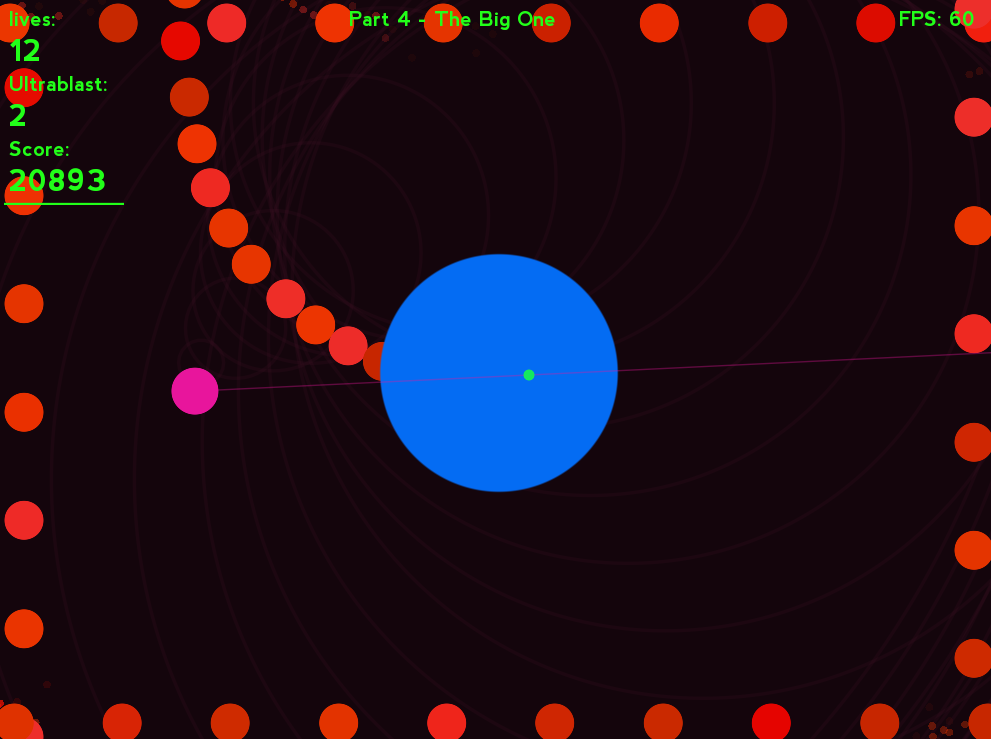
\includegraphics[scale=.3]{ss1}
\centering
\caption{Primeiro chefão do jogo atacando o jogador}
\end{figure}

O jogo, em seu último lançamento, possui 2 dos 5 níveis planejados. Cada nível tem sua própria trilha sonora, e é dividido em quatro partes únicas, sendo a última composta por um \textit{chefão}. \textit{PsyChO: The Ball} possui vários efeitos especiais visuais e sonoros, e abrange 5 tipos de inimigos diferentes para desafiar o jogador.

\begin{figure}[h!]
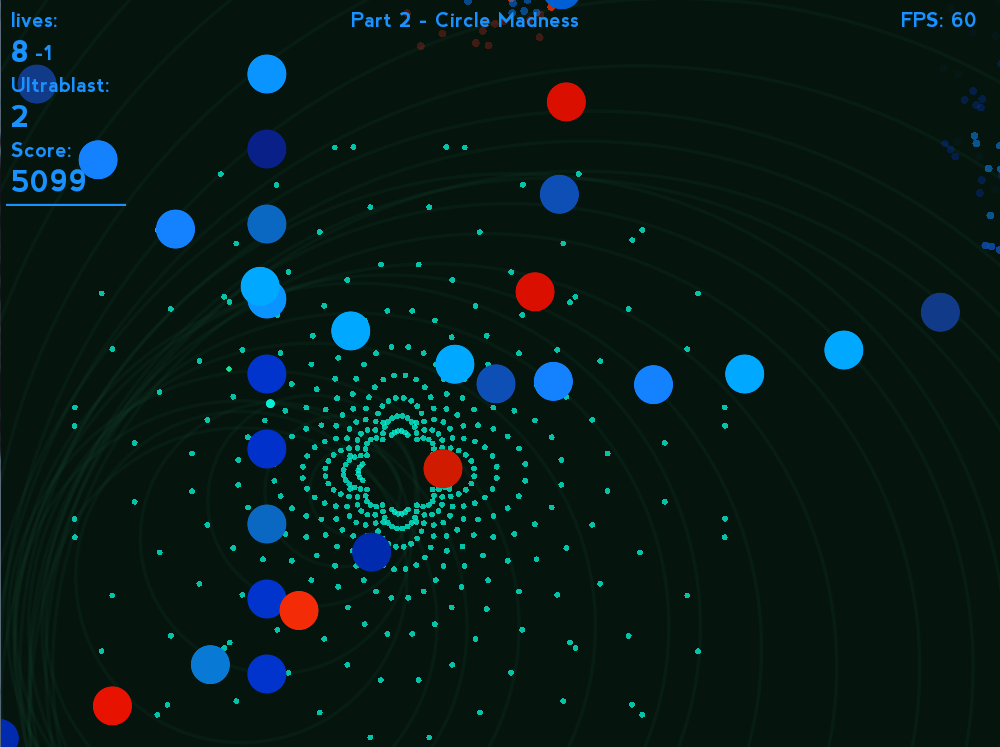
\includegraphics[scale=.3]{ss4}
\centering
\caption{Jogador morrendo para uma onda de inimigos lhe atacando}
\end{figure}

Além disso, o jogo salva as maiores pontuações entre partidas, então jogadores podem sempre tentar superar a pontuação de colegas, ou tentar aumentar seu próprio recorde. O sistema, por rodar níveis através de \textit{scripts}, permite facilmente que usuários criem e joguem seus próprios níveis, sem precisar de muito conhecimento computacional.

% ---------------------------------------------------------------------------- %
\section{Eventos}
\label{sec:eventos}


\begin{figure}[h]
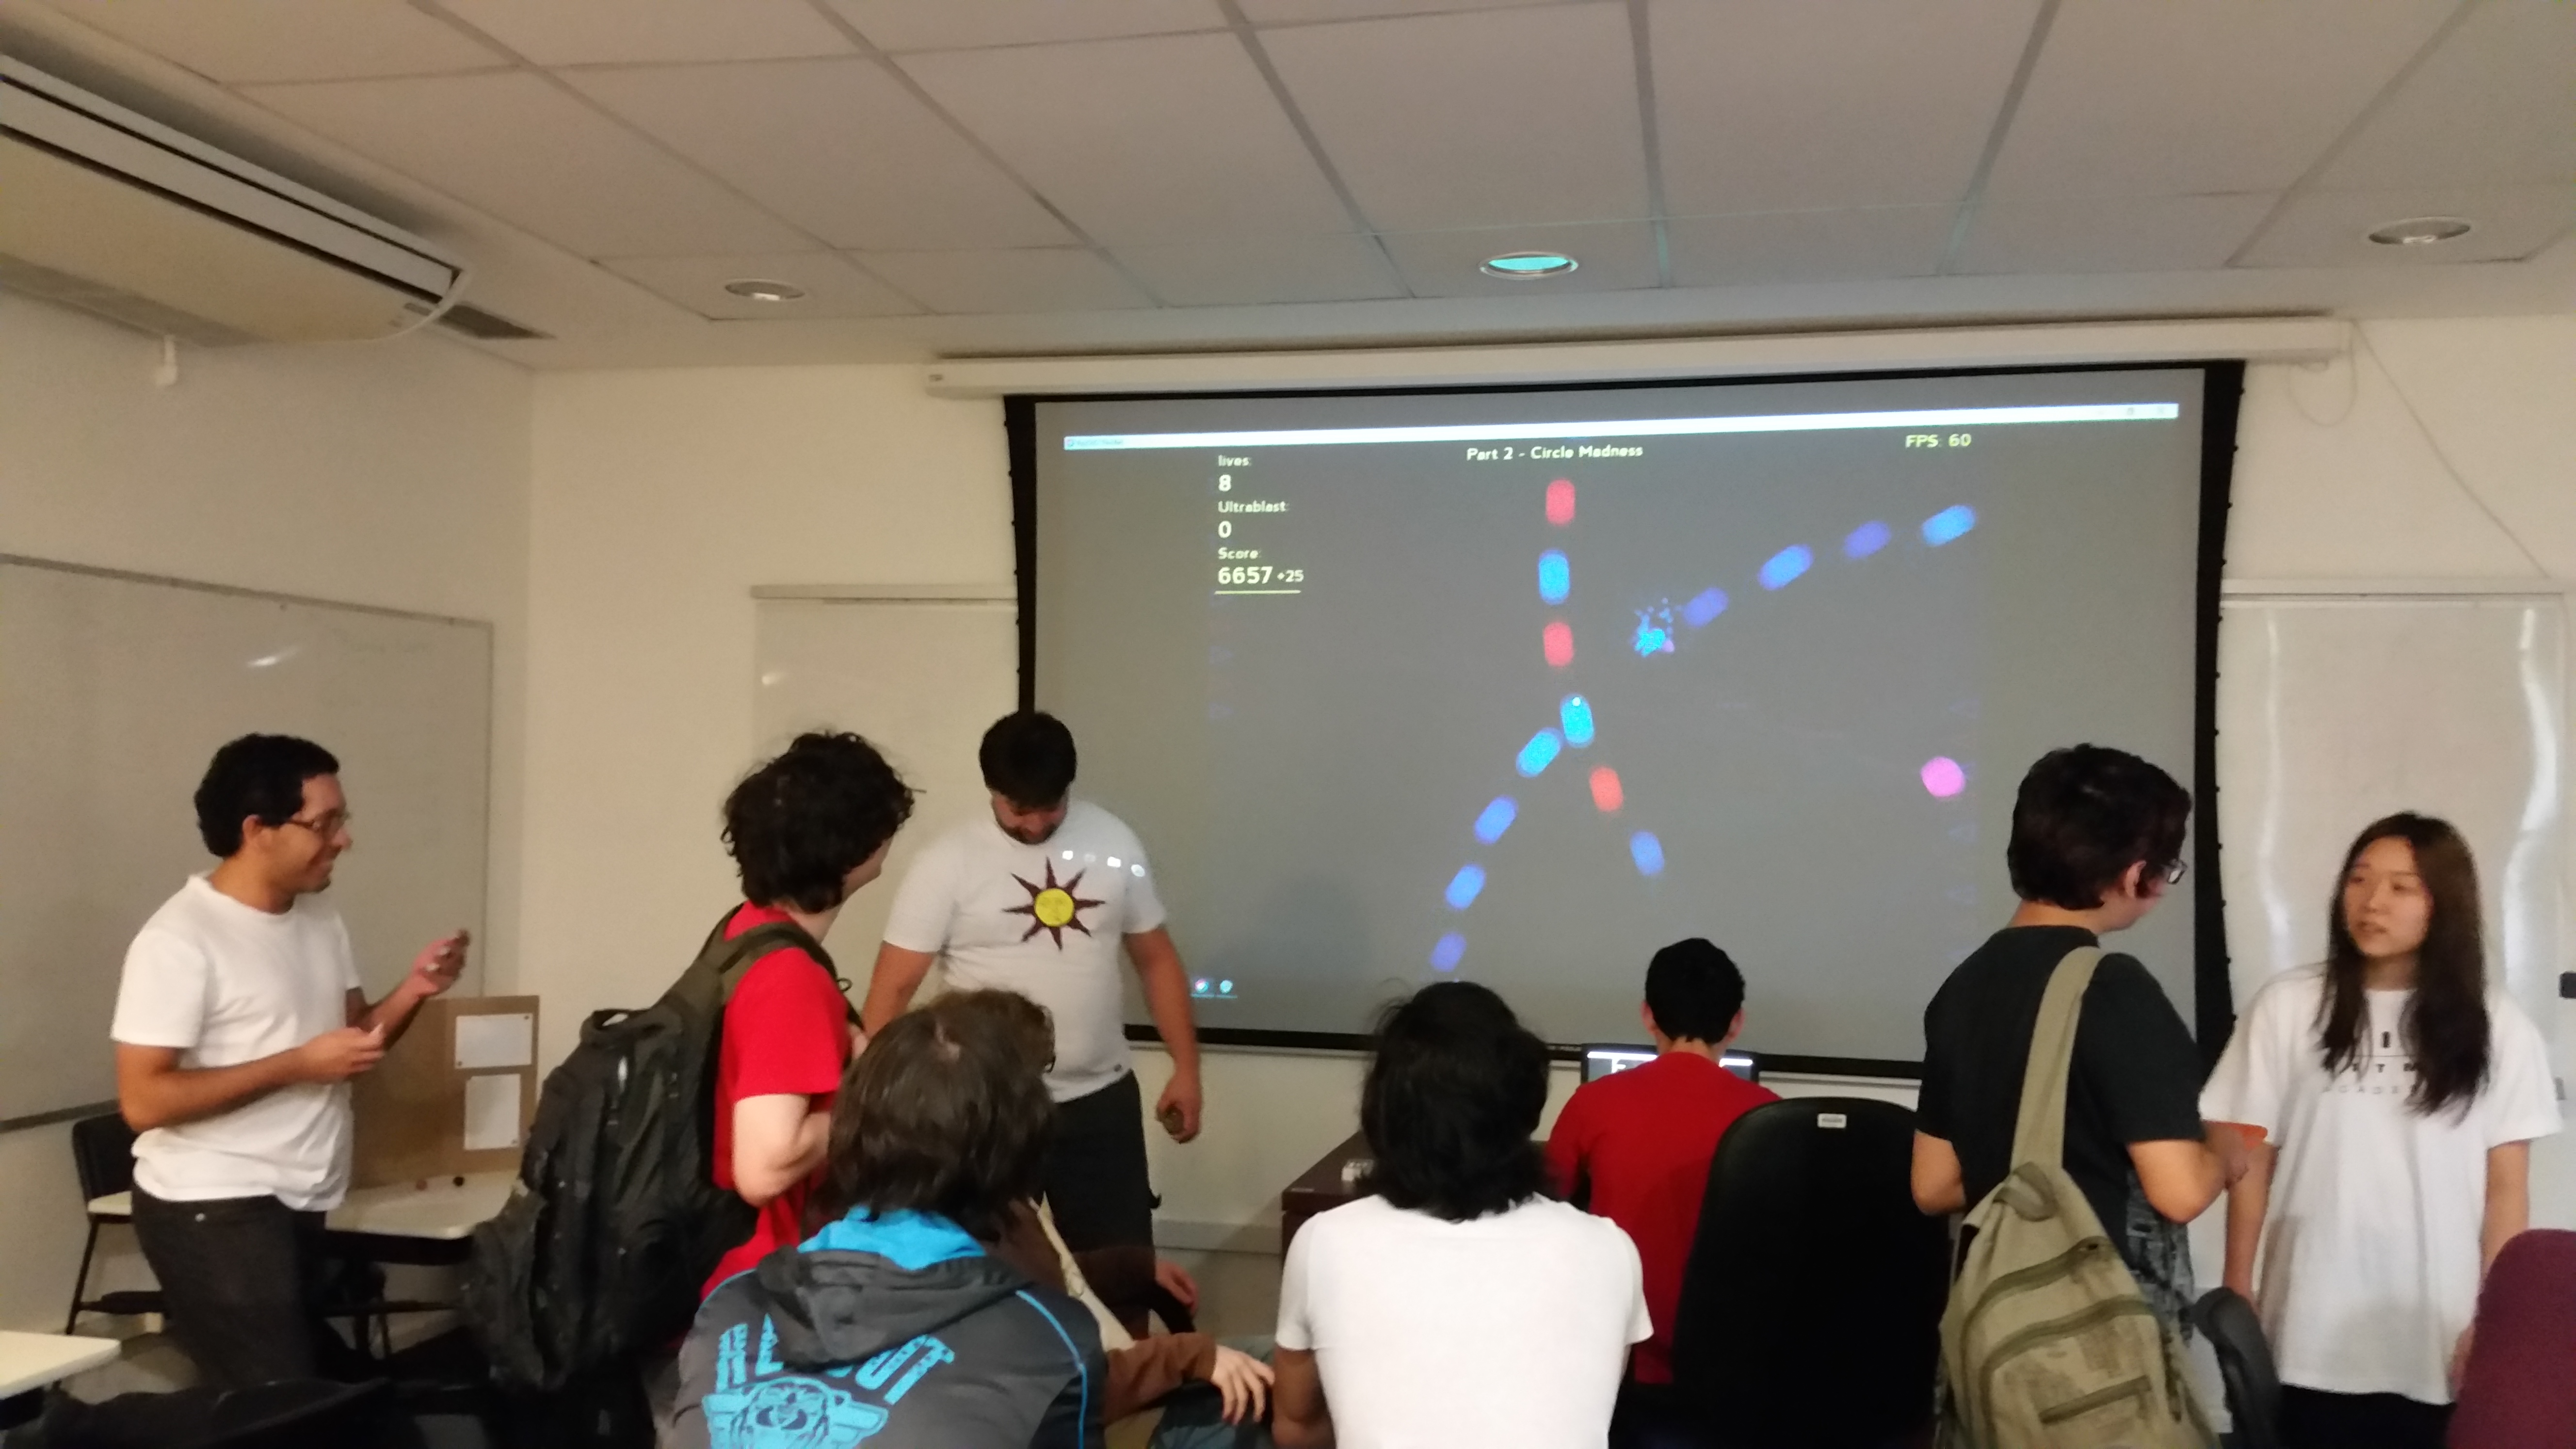
\includegraphics[scale=.06]{letsplay1_2}
\centering
\caption{Evento \textbf{Let's (test) Play!}. No fundo \textit{PsyChO: The Ball} - 02/12/2016}
\end{figure}

A primeira exposição pública de \textit{PsyChO: The Ball} foi em dezembro de 2016, em um evento aberto, organizado pelo grupo \textit{UspGameDev}: \textbf{Lets (test) Play!}. Nele, todos os integrantes do grupo tiveram uma chance de mostrar o progresso de desenvolvimento em seus projetos, para a comunidade \textit{Uspiana}. Desta forma, alunos, professores e funcionários puderam jogar, dar opiniões e, acima de tudo, se divertirem durante uma tarde nos jogos.

Foi um momento marcante no desenvolvimento de \textit{PsyChO: The Ball}, pois receber o \textit{feedback} de outras pessoas tem tanto a utilidade para o aperfeiçoamento do jogo, como traz uma satisfação pessoal, ao ver as pessoas se envolverem num projeto que demorou meses para ser desenvolvido. Uma das maiores mudanças que surgiu nesse primeiro evento foi a implementação do sistema para armazenar pontuações máximas, assim jogadores podiam comparar resultados no jogo entre sí.

O segundo grande evento ocorreu em julho de 2017: \textbf{II Let's (test) Play}. Nesta sequência, foram apresentados mais projetos de membros da \textit{UspGameDev}. Além disso, teve uma quantidade maior de pessoas comparecendo, até mesmo das não atreladas à \textit{Universidade de São Paulo}. Foi possível mostrar todo o progresso no desenvolvimento do jogo nos 6 meses que se passaram, tendo o projeto se fortalecido com todo o \textit{feedback} recebido pelos alunos e professores que quiseram jogar \textit{PsyChO: The Ball}.

\begin{figure}[h!]
  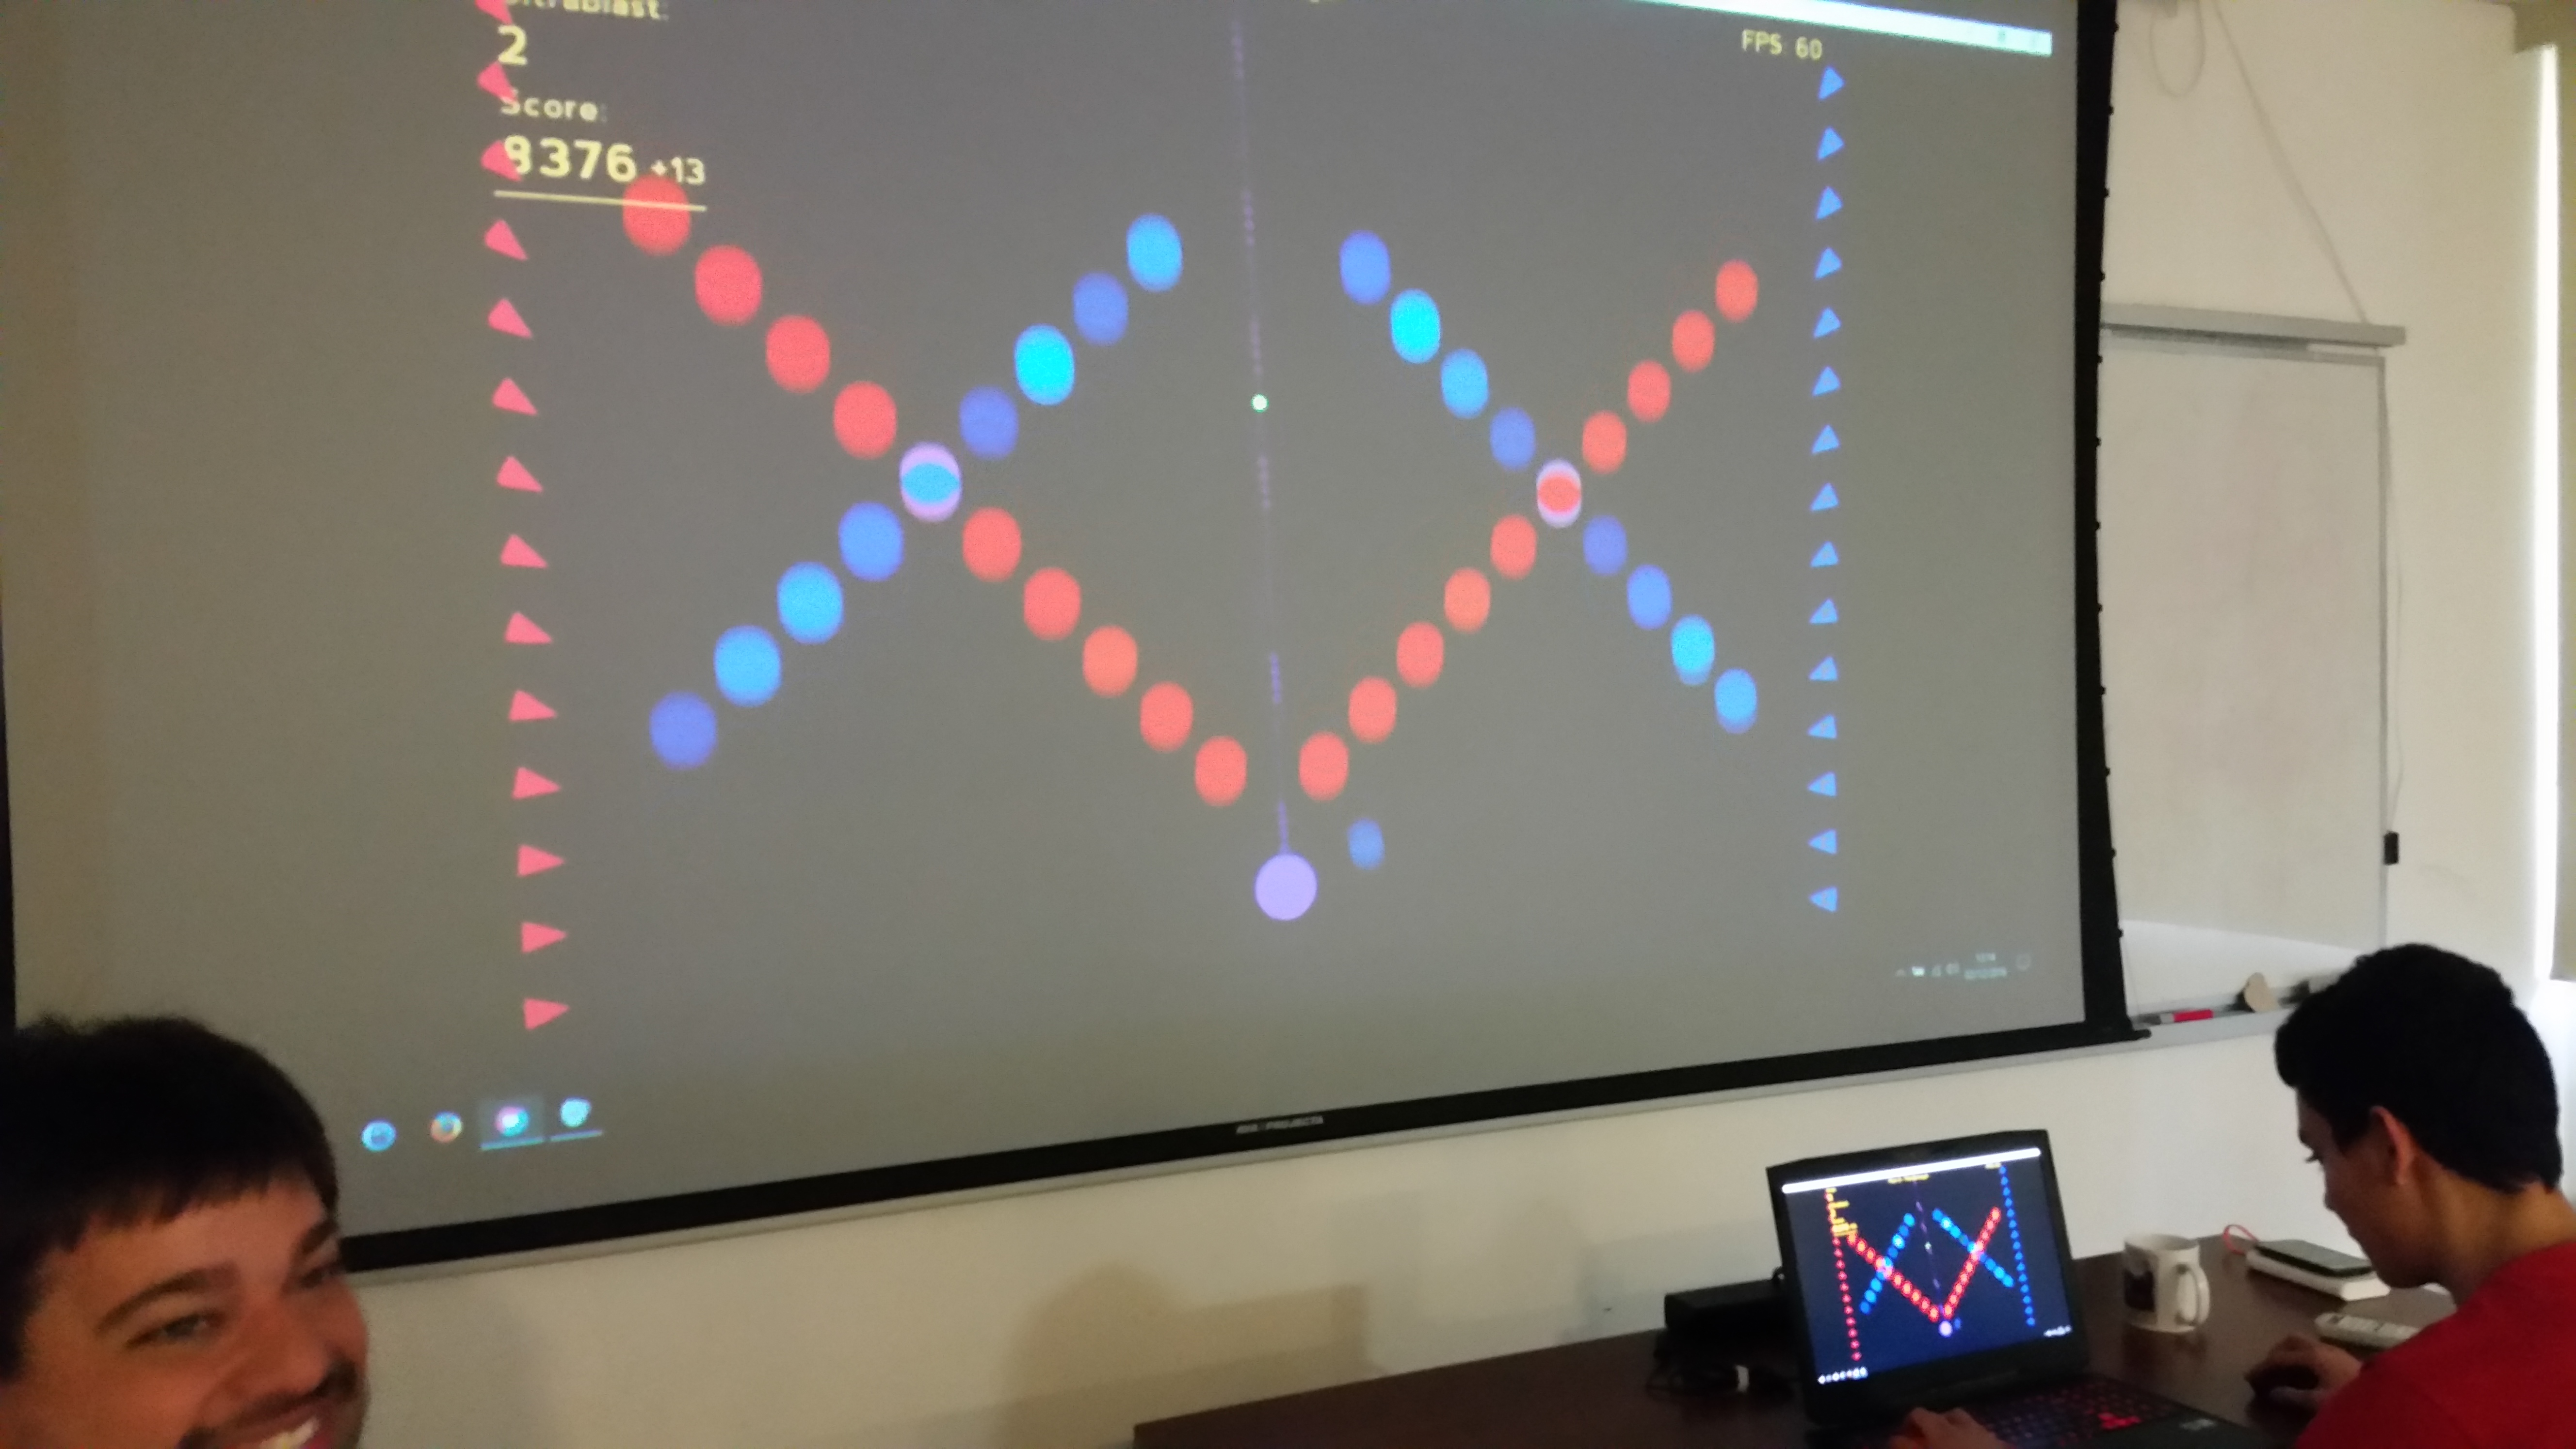
\includegraphics[scale=.06]{letsplay1_1}
  \centering
  \caption{Aluno jogando \textit{PsyChO: The Ball} no \textbf{Let's (test) Play!} - 02/12/2016}
\end{figure}

\begin{figure}[h]
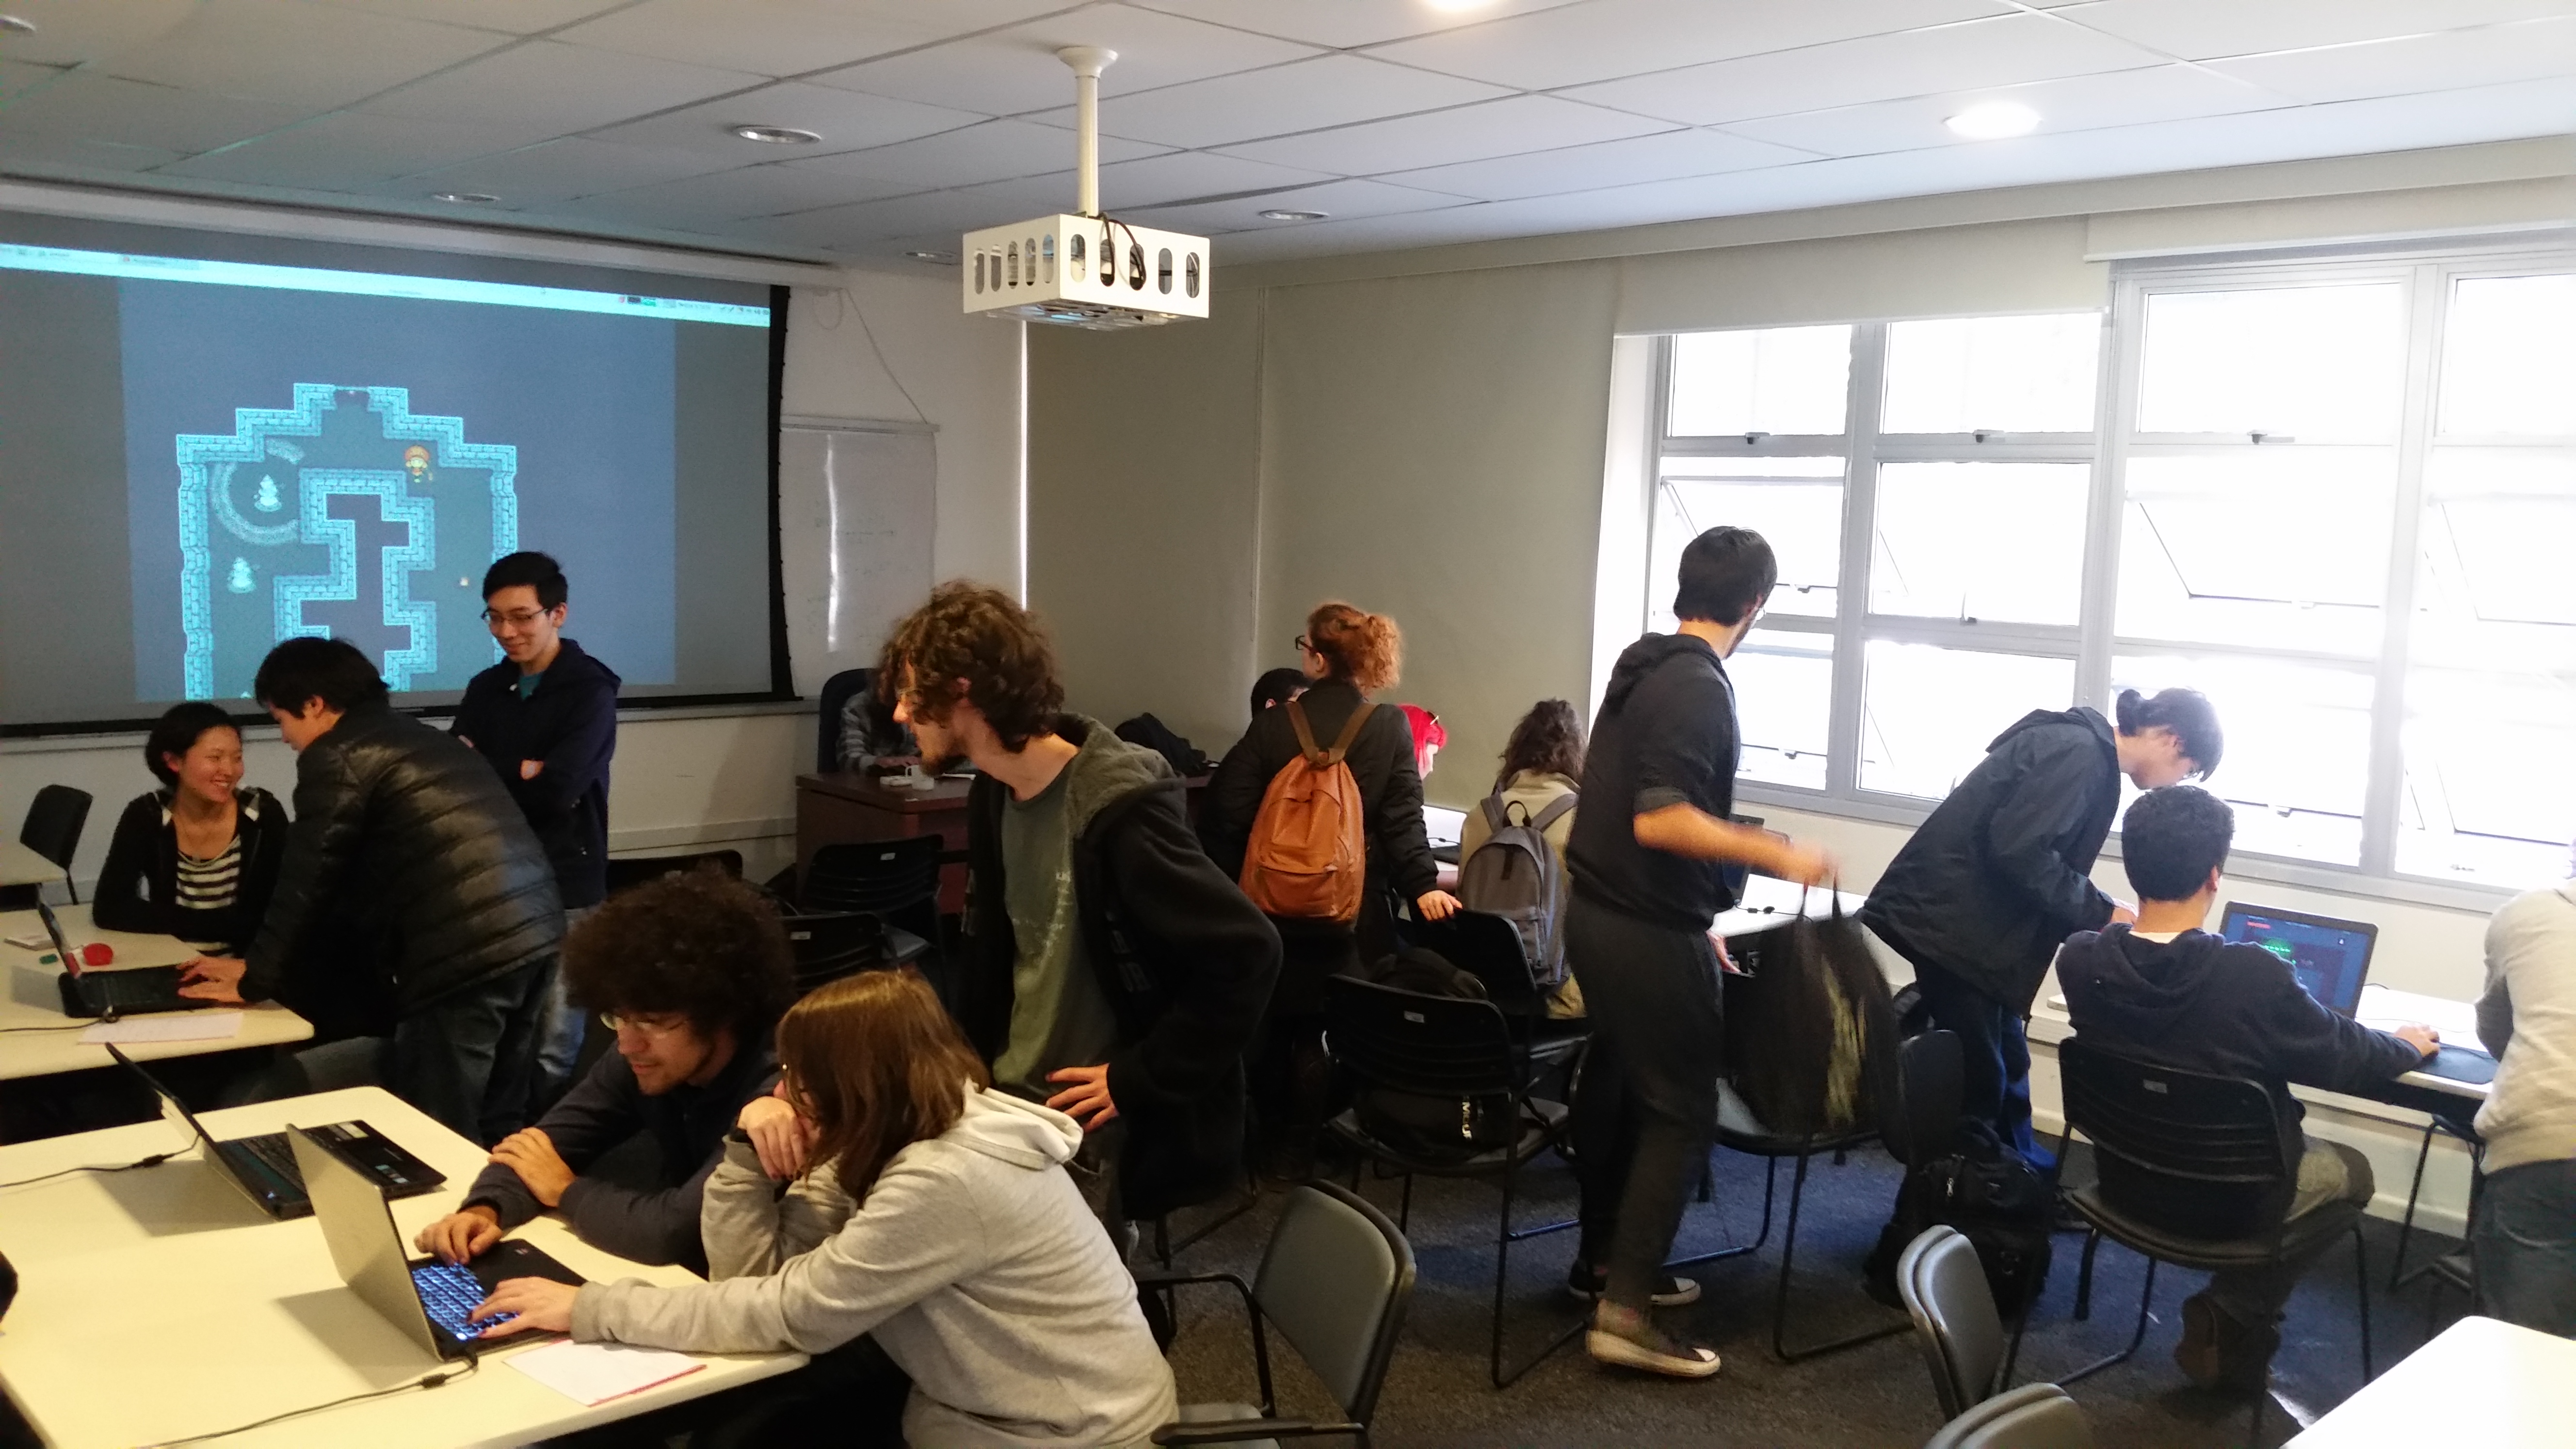
\includegraphics[scale=.06]{letsplay2}
\centering
\caption{Foto do evento \textbf{II Let's (test) Play} - 05/07/2017}
\end{figure}

% ---------------------------------------------------------------------------- %
\section{Como Jogar}
\label{sec:how_to_play}


\textit{PsyChO: The Ball} possui todos seus lançamentos disponiveis \textit{online} em seu próprio repositório, no domínio \textit{Github}:
\\~\\
\url{https://github.com/uspgamedev/Project-Telos/releases}
\\~\\
Neste link é possível encontrar instruções de como instalar e jogar \textit{PsyChO: The Ball} nos sistemas operacionais \textit{Linux} (suporte direto para \textit{distros} baseadas em \textit{Ubuntu} ou \textit{Debian}), \textit{Windows} e \textit{Macintosh}.
\\~\\
Além disso é possível acessar diretamente a versão mais atualizada do código fonte, através da página principal do repositório do projeto:
\\~\\
\url{https://github.com/uspgamedev/Project-Telos/}
